 % !TeX spellcheck = en_GB
\documentclass[12pt,onecolumn,twoside]{layout}
% Use the lineno option to display guide line numbers if required.

\usepackage{setspace}
\usepackage{gensymb}

\title{The German Coal Debate on Twitter: Reactions to a Corporate Decision-Making Policy Process}

% Use letters for affiliations, numbers to show equal authorship (if applicable) and to indicate the corresponding author
\author[a,b]{Yuan Ting Lee}

\affil[a]{Hertie School, Friedrichstr. 180, Berlin 10117, Germany}
\affil[b]{Mercator Research Institute on Global Commons and Climate Change, Torgauer Str. 12 - 15, Berlin 10829, Germany}

% Please give the surname of the lead author for the running footer
\leadauthor{Lee} 

% Please include corresponding author, author contribution and author declaration information
\authorcontributions{}
\authordeclaration{}
\equalauthors{}
%\correspondingauthor{\textsuperscript{1}To whom correspondence should be addressed. E-mail: y.lee@mpp.hertie-school.org}

% Keywords are not mandatory, but authors are strongly encouraged to provide them. If provided, please include two to five keywords, separated by the pipe symbol, e.g:
%\keywords{Keyword 1 $|$ Keyword 2 $|$ Keyword 3 $|$ ...} 

\begin{abstract}
Abstract goes here
\end{abstract}

%\dates{This manuscript was compiled on \today}

\begin{document}
\onehalfspacing
\maketitle
\thispagestyle{firststyle}
\ifthenelse{\boolean{shortarticle}}{\ifthenelse{\boolean{singlecolumn}}{\abscontentformatted}{\abscontent}}{}

\section*{Introduction} \label{sec:introduction}
% [T: 1500, C: 1500]
% Coal exit
Coal combustion contributes to more than a third of today's carbon emissions, and is a major contributor to local adverse effects on the environment and public health.  In line with a global climate ambition to limit the increase in global average temperature to well below 2 \si{\degree}C as denoted by the Paris Agreement, all countries must achieve a rapid decarbonisation of all sectors by the middle of this century \cite{Figueres2017}. Much of the research on this topic has focused on the energy sector due to its high remaining emissions but comparatively cheap abatement potential \cite{Armstrong2016}. 

\subsubsection*{The problem with coal}
Indeed, coal-fired power plants remain one of the key drivers of global warming \cite{Edwards2019,Zhao2019} There are also  additional environmental costs in the form of airborne pollutants, which in turn have a negative effect on human health as well. This leads to coal having a high environmental and social cost. Lignite has the highest environmental cost in electricity generation, at 20.81 Euro Cents/KWh, followed by hard coal at 18.79 Euro Cents/kWh [CITE]. Studies show that phasing out coal yields substantial local environmental and health benefits that outweigh direct policy costs \cite{Rauner2020}. As a result, a coal phase-out presents an attractive option for coal-intensive countries to reduce their carbon emissions.

When referring to coal, there are two different types that are often referred to: hard coal and lignite. Lignite, sometimes referred to as brown or soft coal, has a lower carbon content and fuel value than hard coal, and is not mined below ground like hard coal but rather in opencast mines \cite{Appunn2019}. 

\subsubsection*{Coal in Germany}
Germany is the world's largest producer of lignite, where lignite and hard coal provide almost 40\% of electricity in the country. One of the reasons for continued lignite-fired power production in Germany is the access to lignite resources in the country, concentrated in 3 areas: the Rhineland, Lusatia, and Central Germany \cite{AgoraEnergiewende2019}. 

Germany has experienced a coal phase-out before, with that of the mining of hard coal. From 1958, hard coal production and employment in Germany started to decline due to a price drop that resulted from the liberalisation of coal prices that was previously regulated by the European Coal and Steel Community (ECSC), the predecessor of the European Union (EU)) \cite{Oei2019}. Domestic hard coal faced fierce competition from other comparatively cheaper energy sources: imported coal from overseas, as well as imported oil.  In 2007, with the growing influence of the EU, Germany ended its subsidies for hard coal production, and the last active hard coal mine in Germany was closed at the end of 2018 \cite{Appunn2018}, bringing an end to a long history of hard coal mining in the country. Hard coal-fired power production, however, remains active in the country, with imported coal coming from Russia, Colombia, and the United States [CITE]. 

The phase-out of hard coal mining in Germany was thus largely economically motivated. In contrast, lignite mining remains a profit-making business in Germany, with the opencast pit mines located near the power plants \cite{Appunn2019}. As a result, in order to phase out lignite mining in Germany, it has to be directed by the government as part of its environmental and energy policies. Consequently, the current German government comprising the Chancellor Angela Merkel's conservative CDU/CSU\footnote{Christian Democratic Union, Christian Social Union} and the Social Democrats (SPD) agreed to set up a special commission consisting of different stakeholders to manage a coal phase-out in Germany. This was formally introduced in their coalition contract in 2018 \cite{Wehrmann2018}.  

\subsubsection*{Multi-stakeholder commissions}
Multi-stakeholder commissions present an important instrument for incorporating external interests into political decision-making. It can be seen as an element of ``negotiation democracy'', whereby the stakeholders in the commission decide on a policy outcome, or deliver policy recommendations via deliberations and negotiations. Depending on the policy field, representatives of business, science, the social partners, churches, associations and societies can be appointed and thus accelerate the later public discussion. \cite{Siefken2016}

% Examples of multi-stakeholder commissions in policy-making
The use of multi-stakeholder commissions have been used in environmental policy decision-making in Germany before, in the planning of a nuclear phase-out. Although an exit from nuclear power had been previously agreed to by the federal government, an external expert commission, titled the ``Commission to Review the Financing for the Phase-out of Nuclear Energy'', was set up in 2015 to manage the financing of the nuclear phase-out. The commission was tasked with ensuring that the ``polluter pays'' principle (where the polluters refer to nuclear power plant operators) was upheld and that taxpayers would not end up footing the cost of decommissioning nuclear plants and storing nuclear waste \cite{Appunn2017}. 

\subsubsection*{The German Coal Commission}
The coal commission, formally known as the Commission on Growth, Structural Change and Employment, is another example of a multi-stakeholder commission. It was set up by the German government in 2018 under the Federal Ministry for Economy and Energy (BMWi), and was tasked with developing an overarching approach to managing the coal phase-out’s technical, legal, economic and social impacts. This was done so under the backdrop of Germany looking likely to miss its 2020 climate targets, and increasing international pressure for greater climate action [CITE]. 

The coal commission was given the mandate to develop a plan to gradually reduce and shut down coal-fired power generation, including a completion date and the necessary accompanying legal, economic, social, renaturalisation and structural measures. \cite{Groll2019} The commission comprised key stakeholders from businesses and industries, the trade unions, energy industry, as well as representatives from coal-mining regions in Germany, the Parliament, administration, environmental NGOs, and scientists \cite{AgoraEnergiewende2019}. 

% Process of the commission
The Commission was formally established on 6 June 2018, and first met on 26 June 2018. This was followed with nine meetings on roughly a monthly basis until the closing meeting on 25 January 2019. In addition to discussions between members, during the initial meetings, the Commission listened to technical experts from the Federal Government, the Federal States, industry, trade unions, the sciences, and civil society \cite{Wehrmann2018}. On 26 January 2019, the Commission unveiled its findings in a final report that was submitted to the federal government in February 2019. One of the key recommendations from the commission's report was to set a deadline to phase-out coal -- by shutting down existing coal-fired power plants step by step until 2035, or 2038 by the latest. In addition, the commission also recommended to support the affected regions by the coal phase-out with a structural transition fund amounting around 40 billion euros \cite{Egenter2019}. Following the release of the coal commission's report, the German cabinet adopted its coal exit law on 29 January 2020, largely following the recommendations of the coal commission, and clearly distinguish the pathways for hard coal and lignite phase-out in Germany \cite{Wettengel2020}. 

% Link to public opinion 
Criticisms have emerged about the process and outcome of the coal commission, namely that the recommendations that it propose are not consistent with the Paris Climate Agreement \cite{klimareporter2019a}, nor did it meet Germany's own climate targets. It has been framed as a victory for the coal regions and industries, but the final report, dubbed the ``coal compromise'', has also been criticised by environmental activists for not reflecting a consensus \cite{klimareporter2019,endegelaende2019}. The approach of installing a multi-stakeholder commission has also been criticised, as the commission presented its recommendations as a direct policy prescription, which falsely assumes that such a prescription is value-neutral. Further, it has been suggested that the commission should have been mandated to present several path options including their implications as opposed to one clear-cut phase-out solution \cite{Kowarsch2019}.     

The process of the German coal commission thus presents a unique situation for analysis: is there a relationship between the seemingly ``corporatist'' process of such a multi-stakeholder commission and public opinion? Did the coal commission, through its process of incorporating members representing different interests, help reach consensus in the wider public as well, or did its final report reflect a lack of consensus, as claimed by its critics?

\subsubsection*{Public Opinion and Social Media Data} % Twitter and social media data
Public opinion is traditionally measured from conducting surveys, of which the survey response samples are then weighted proportionally to represent the views of the population. However, some of the disadvantages of these methods are that they are extremely resource intensive. They are also typically conducted over a lengthy period of time, resulting in it being difficult to extract real-time responses and opinions on trending issues \cite{Klasnja2018}. 

One alternative to this is to measure public opinion using social media data. Social media provide an opportunity to examine public opinion without any prompting or framing effects from analysts. The data is also fine-grained and allows for detailed temporal analysis, which is useful for tracking decision-making processes such as the coal commission, which span a period of time with different significant events occurring at different stages \cite{Klasnja2018}. 

Here, tweets from Twitter are used to represent public opinion on social media, in part due to their high granularity which allows for observations on swiftly changing temporal patterns on topic salience. In addition, Twitter is commonly used as a source of information about breaking news events, and journalists and traditional media often solicit feedback from the public through social media. This presents an opportunity to study the public opinion about a topic through looking at tweets. 

\section*{Related Work} \label{sec:relatedwork}
% [T: 750, C: 380]
Twitter has been used to explore a variety of social and linguistic phenomena \cite{Cao2012, Lin2013, Lin2014}, and has also been used in the study of politics, in political responsiveness \cite{Barbera2019}, and also in political attention \cite{Hemphill2014, Shapiro2017}. It is also often used in the analysis of public opinion with regards to politics \cite{DiGrazia2013, Vaccari2013, Barbera2016}.

Twitter has been used as a medium to analyse human sentiment through the analysis of variations in the frequency of specific words used by individuals. In \cite{Dodds2011}, Dodds et. al. develop a tool for measuring expressed happiness via positive and negative sentiment in large-scale text corpora. Since its development, the tool, named the ``hedonometer'', has been implemented in studies involving the happiness of cities and states \cite{Bliss2012}, the happiness of the English language as a whole \cite{Kloumann2012}, the relationship between individuals' happiness and that of those they connect with \cite{Mitchell2013}, and as a method of unsolicited public opinion polling on climate change \cite{Cody2015}. Other examples of applying sentiment analysis to tweets include studying public perception of climate change through temperature anomalies \cite{Moore2019}. 

In the previous paragraph, the category of sentiment analysis used is that of a dictionary-based method, which involves scoring words and sentences based on an existing dictionary with sentiment scores for individual words, followed by some aggregation. However, there are other methods of using sentiment analysis, namely involving classification methods. This may involve the use of machine algorithms, which train on an input of manually classified data, in order to classify a larger set of un-labelled data. This method is used in \cite{Stukal2019}, which uses neural networks to classify the political orientation of ``bots'' (automated posters) on Twitter. 

% network analysis
Other work have looked at the debate on Twitter on climate change. In \cite{Williams2015}, Williams et. al. conduct a network analysis on the climate change debate on Twitter, classifying active users in the dataset based on their expressed attitude towards climate change - as ``activists'', ``sceptics'', or ``neutral''. The networks were then constructed by looking at the frequency of tweets, as well as the interactions between the different user groups. The authors found that most users only interacted with other like-minded users within the same community. However, they also found communities with interactions from different user groups, where messages between like-minded users carried positive sentiments, while messages between sceptics and activists carried negative sentiment.

\section*{Task} \label{sec:task}
% [T: 300, C: 280]
This project aims to identify whether there was an effect on public opinion on the German coal exit throughout the entire decision-making process of the coal commission. Specifically, this project seeks to answer the question: did the establishment of a multi-stakeholder, corporatist process like the Coal Commission lead to societal consensus? To do so, significant events throughout the coal commission process have to be identified and a measure for public opinion has to be designed. Here, public opinion can be abstracted from sentiment analysis of tweets made throughout the timeline of the coal commission's lifetime using dictionary methods and polarity weighting. A suitable dictionary for the analysis of the German language also has to be used. 

In addition, in order to understand the public reaction to the deliberative process of the coal commission, it is necessary to understand the broader coal debate on Twitter and how Twitter users on the platform engage in the coal debate -- both on the topic in comparison to other debates, as well as with fellow users on the same topic. This involves designing an adequate search strategy for collecting tweets on both the coal commission, but also the broader coal exit discussion, and also the climate discussion on Twitter as a baseline comparison for the coal debate. 

Finally, in order to answer the question of whether a consensus was reached in the public across the process of the coal commission, comparison periods have to be defined, and a measure for measuring consensus has to be drawn up as well. This can be done either by looking at variation in sentiment scores over time, or via other methods such as analysis of interaction networks between Twitter users. 

\section*{Data} \label{sec:data}
% [T: 500, C: 280]
The data used in this project was collected via a two-part process, using two python packages: \texttt{twint} to download the tweets based on specific queries, and \texttt{tweepy} to populate the tweets with extended tweet information. %be more specific and clear here

The selection process for choosing tweets to analyse stems from the research question at hand, which is to understand the greater coal debate in Germany on Twitter. The final collection of tweets thus include two sets of tweets collected using two different search strategies. The first search strategy includes terms that directly relate to the coal exit in Germany - \{Kohlekommission, Kohleausstieg, Kohlefrei\}.\footnote{Translation: Coal commission, Coal exit, Coal free}

The other set of tweets is obtained from a general search for tweets on coal (``Kohle''), which are then filtered by the inclusion of relevant hashtags in the text of the tweets. These relevant hashtags are obtained by conducting a frequency analysis of all hashtags that appear in ``Kohle'' tweets, and manually selecting the top hashtags that are related to coal in climate policy. These hashtags are:  \{\#Klimaschutz, \#Hambacherforst, \#Hambibleibt, \#endcoal, \#fridaysforfuture, \#klimawandel, \#klima, and \#endegelaende\}.\footnote{Translation: Climate policy, Hambach Forest, Stay Hambach (forest), Climate Change, Climate, End of the Site} 

The dates for the queries are limited to between 2017-01-01 and 2020-02-29. The two collections are then combined and duplicates are removed, and the final set is then filtered for tweets in German, which can be obtained as a result from querying the Twitter API. In the data set, each retweet is counted as a separate tweet, and is denoted as a retweet in the text field by beginning with ``RT''. 

In addition to the above set, another set of tweets was collected to use as a baseline for comparison. This set includes the search terms of \{Klima, Erderwärmung, globale Erärmung, Treibhauseffekt\}\footnote{Translation: Climate, Earth warming, Global warming, Greenhouse effect}.

% insert figure on data collection here

\begin{figure} 
	\begin{center}
		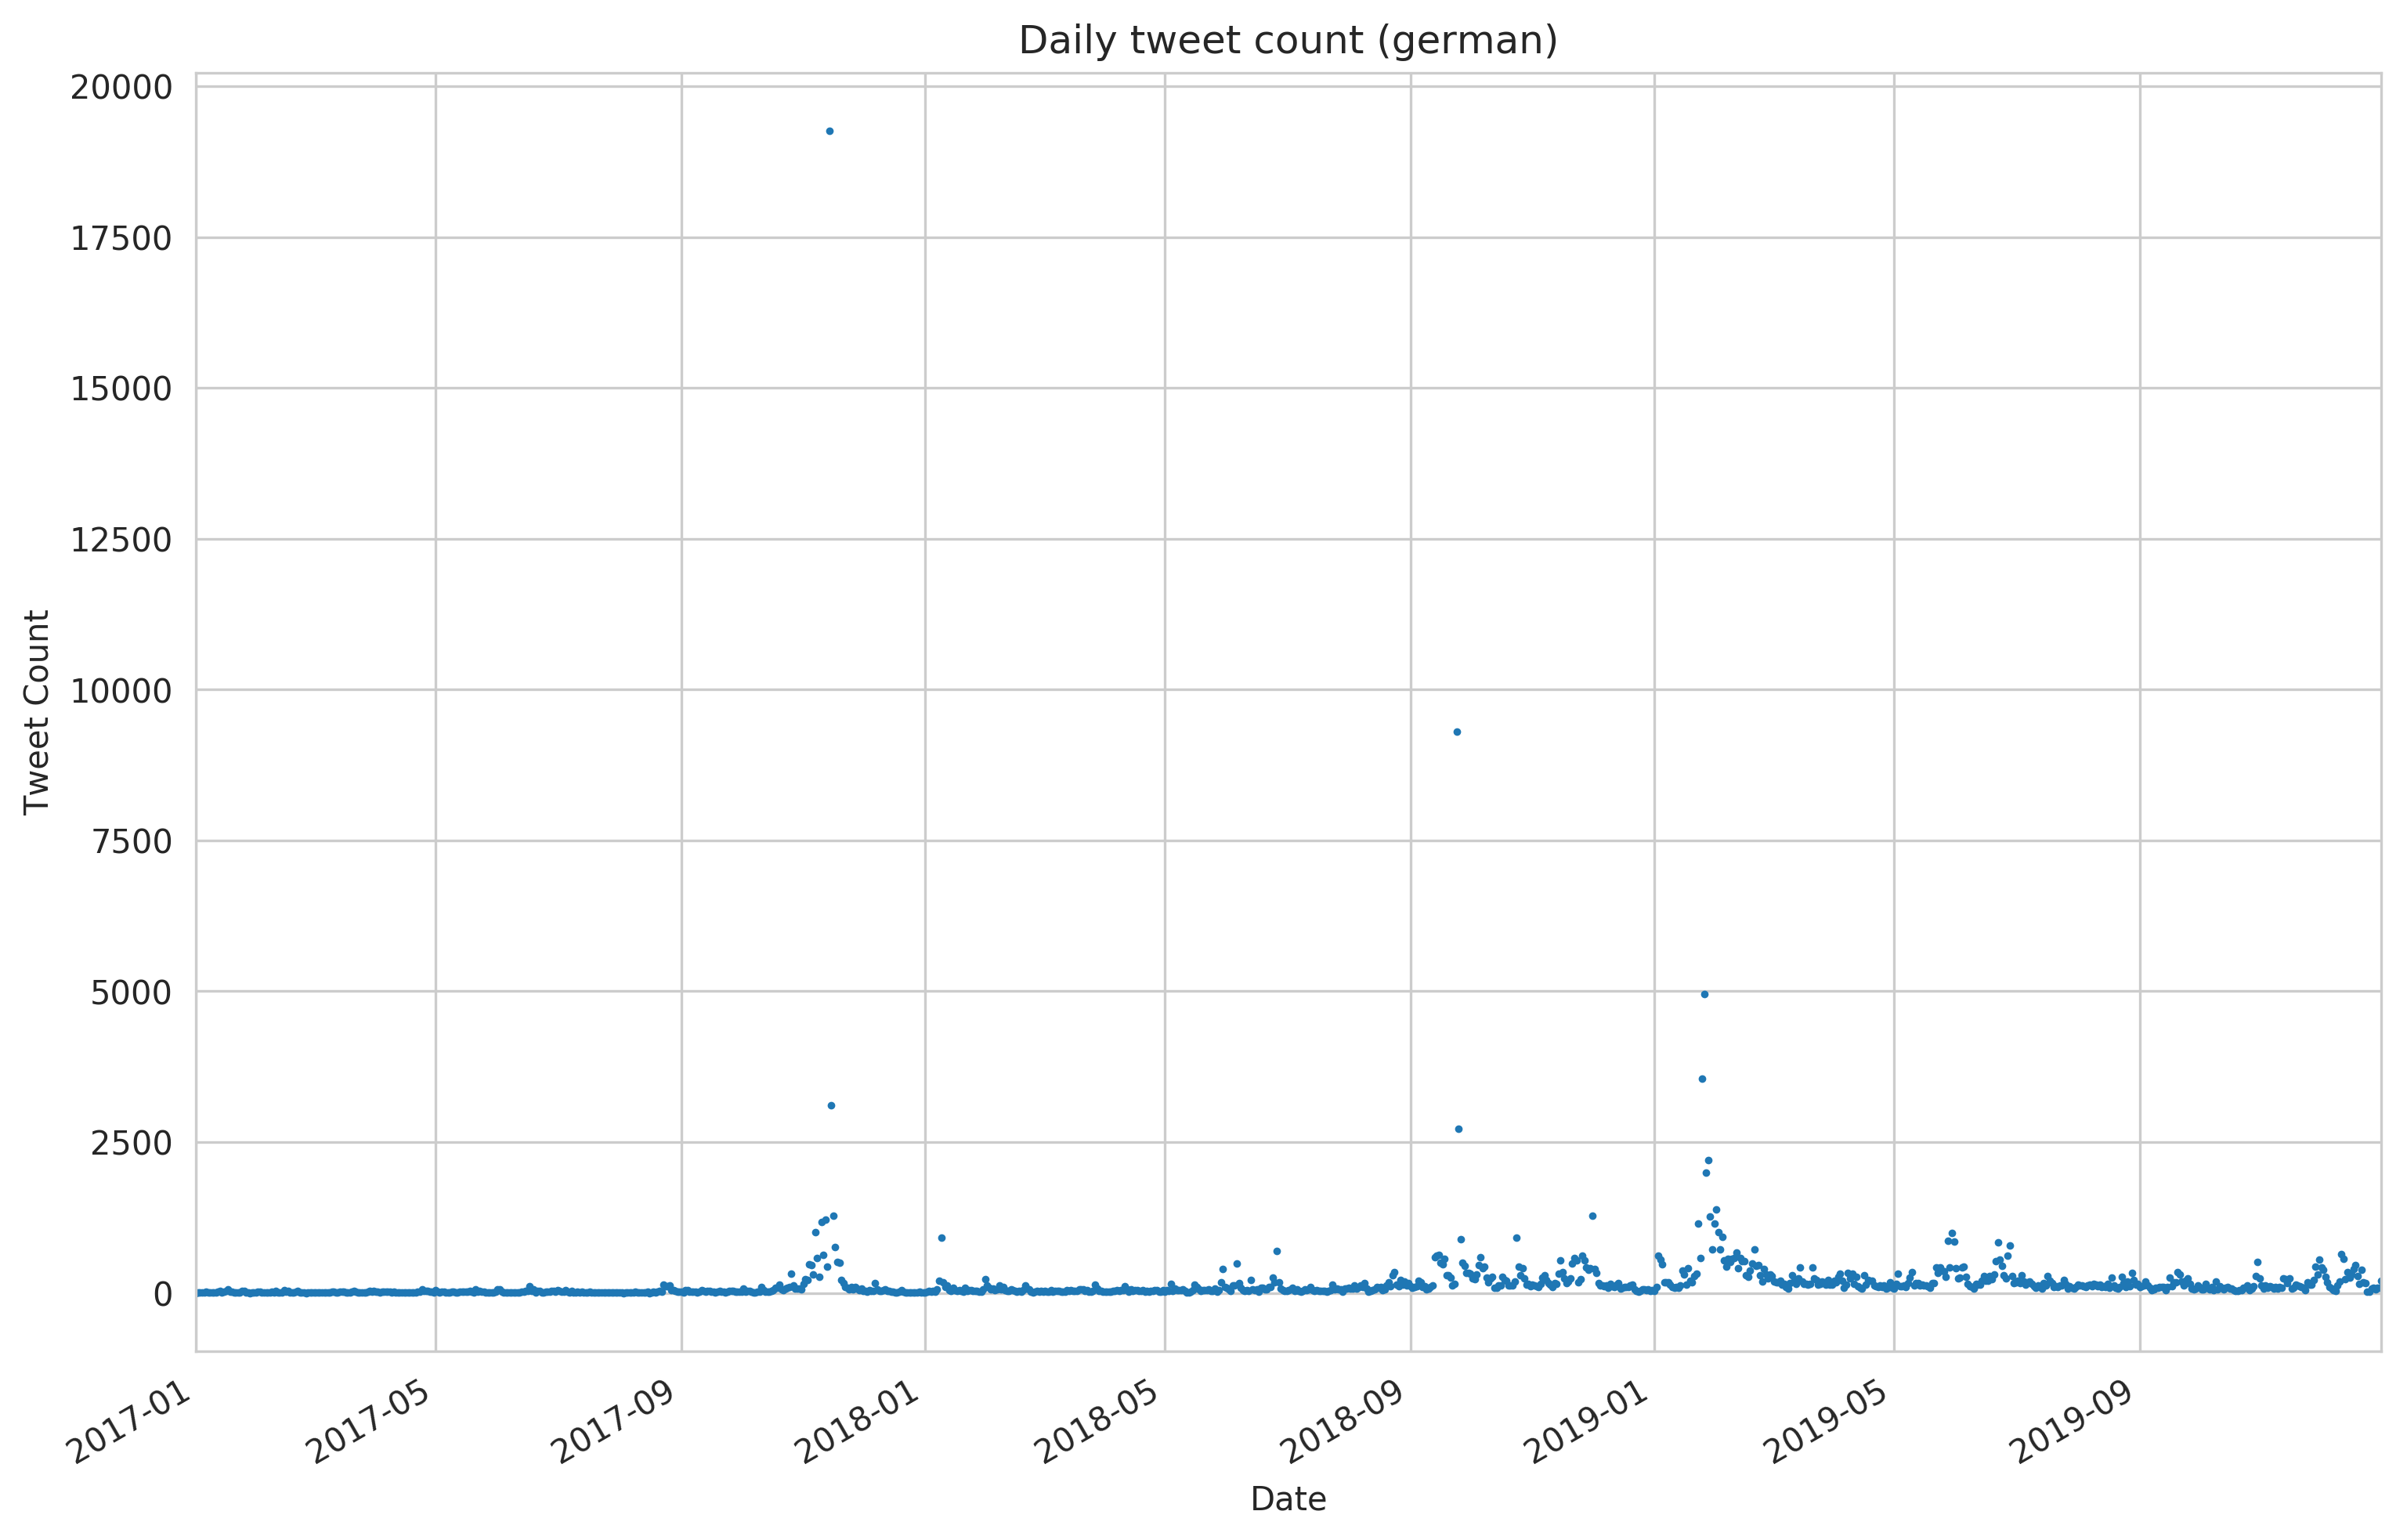
\includegraphics[width=0.75\linewidth]{figures/sa_tweet_frequency_zoom2}
	\end{center}
	\caption{Daily frequency of tweets in combined dataset over coal commission process}
	\label{fig:tweet_frequency}
\end{figure}

\section*{Method} \label{sec:method}
% [T: 800, C: 750]
\subsection*{Sentiment Analysis}
% Explanation of sentiment analysis 

Sentiment analysis refers to the use of natural language processing and text analysis to systematically identify and extract affective states and subjective information in text. % cite?

The dictionary used is SentiWS, a publicly available German-language resource for sentiment analysis \cite{REMUS10.490}. Entries in the SentiWS dictionary set have four components: the word, its Part of Speech (POS) tag, a polarity weight, and inflections associated with the word, as seen in Fig. \ref{fig:sentiws_example}. The semantic orientations of the words are obtained from three different sources with manual revision. 

The weights of word entries in SentiWS are retrieved using a method known as \emph{Pointwise Mutual Information} (PMI), first suggested in \cite{church-hanks-1990-word}. This approach was successfully re-used for sentiment analysis -- the determination of the semantic orientation and the strength of adjectives -- in \cite{Turney2002} and \cite{Turney2003}, where semantic orientation is inferred from \emph{semantic association}. The semantic orientation \(SO\) of a given word \(w\) is calculated from the strength of its association \(A\) with a manually-selected set of positive seed words \(P\) minus the strength of its association with a set of negative seed words \(N\) (cf. Equation \ref{eq:semantic_orientation}). 

\begin{equation}
\label{eq:semantic_orientation}
\text{SO-A}(w) = \sum_{p \in P}A(w,p) - \sum_{n \in N}A(w,n)
\end{equation}

The word \(w\) is classified as having a positive semantic orientation when SO-A(\(w\)) is positive and a negative semantic orientation SO-A(\(w\)) is negative. The absolute value of SO-A(\(w\)) can be considered the strength of its semantic orientation. 

Parallel to the paradigms in \cite{Turney2003}, SentiWS uses a set of German seed words, from which the semantic associations \(A(w,p)\) and \(A(w,n)\) are calculated using PMI (Equation \ref{eq:pmi}): 

\begin{equation}
\label{eq:pmi}
\text{PMI}(w_1,w_2) = \log_2\left(\frac{P(w_1 \& w_2)}{P(w_1) \cdot P(w_2)}\right)
\end{equation}
where \(P(w)\) is the probability that \(w\) occurs and \(P(w_1 \& w_2)\) is the probability that \(w_1\) and \(w_2\) co-occur. The probabilities were estimated using frequencies and co-occurrence statistics on an internal German-language corpus by the creators of SentiWS consisting of approximately 100 million sentences. The final weights are then scaled to the interval of [-1;1] and rounded to 4 decimal places with +1.0 being absolutely positive and -1.0 being absolutely negative.

\begin{figure} 
	\begin{center}
		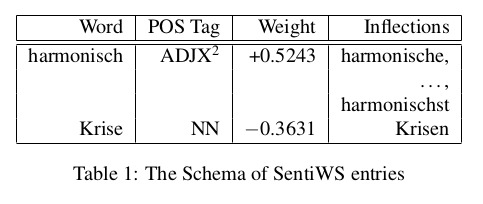
\includegraphics[width=0.5\linewidth]{figures/sentiws_example}
	\end{center}
	\caption{Example of scoring a tweet using the polarity weighting of words from SentiWS}
	\label{fig:sentiws_example}
\end{figure}

To obtain the sentiment score of a tweet, denoted by \(s_{tweet}\), the following formula is used: 

\begin{equation}
\label{eq:word_score}
s_{tweet} = \frac{\sum_{i=1}^{n} s_i f_i}{\sum_{i=1}^{n} f_i}
\end{equation} 
where \(s_i\) is the polarity weighting score of a word given in SentiWS, and \(f_i\) is the frequency of occurrence of the word in the tweet. 

\begin{figure} 
	\begin{center}
		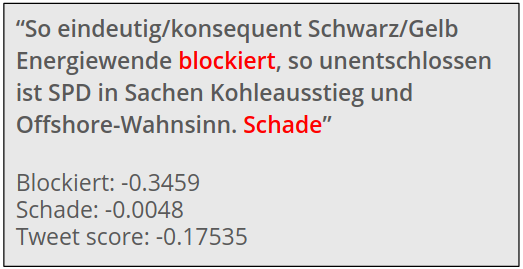
\includegraphics[width=0.5\linewidth]{figures/sentiws_example_use}
	\end{center}
	\caption{Schema of SentiWS entries}
	\label{fig:sentiws_example_use}
\end{figure}

Fig. \ref{fig:sentiws_example_use} shows an example of how the polarity weights from the SentiWS dictionary is used to score a tweet from the coal dataset\footnote{Translation: As unambiguously/consistently black/yellow as the energy turnaround is blocked, so indecisively is the SPD on the coal exit and offshore madness. A pity}. The words ``blockiert'' and ``schade''\footnote{Translation: Blocked, Pity} are the only two words that have non-zero polarity weighting scores in the dictionary, so the sum of the scores of the two words is taken and averaged over the number of scored words (2 in this tweet) to arrive at a average tweet sentiment score of -0.175. 

\subsection*{Word Shift}
% Explanation of word shifts
Building upon the analysis of tweet sentiment scores, word shift graphs represent a measure of the variation between the sentiment scores of two sets of texts. In these graphs, words are ranked by their descending absolute contribution to the change in average valence, between two sets of texts. 

As tweets comprise words, the approach for finding the absolute contributions will be conducted on the word-level. If we consider two sets of texts, \(T_{ref}\) (reference) and \(T_{comp}\) (comparison) with average scores of \(s_{\text{avg}}^{\text{ref}}\) and \(s_{\text{avg}}^{\text{comp}}\) respectively, to compare both texts, we write: 

% need to modify eq so that is either represents entire text set i.e. with average score, or for a single word 	
\begin{equation}
\label{eq:text_difference}
T_{comp} - T_{ref} = \frac{\sum_{i}^{N} s_i f_i^{\text{comp}}}{\sum_{i=1}^{N} f_i^{\text{comp}}} - \frac{\sum_{i,ref}^{N} s_i f_i^{\text{ref}}}{\sum_{i=1}^{N} f_i^{\text{ref}}}
\end{equation} 	
where \(s_i\) is the polarity weighting score of a word given in SentiWS, and \(f_i\) is the frequency of occurrence of the word in the entire text set. 

Equation \ref{eq:text_difference} shows the difference between the normalised score product of each word in the two text sets, and the absolute numbers are then ranked. 

 

\section*{Results} \label{sec:results}
% [T: 3K]
\begin{figure*}
	\begin{center}
		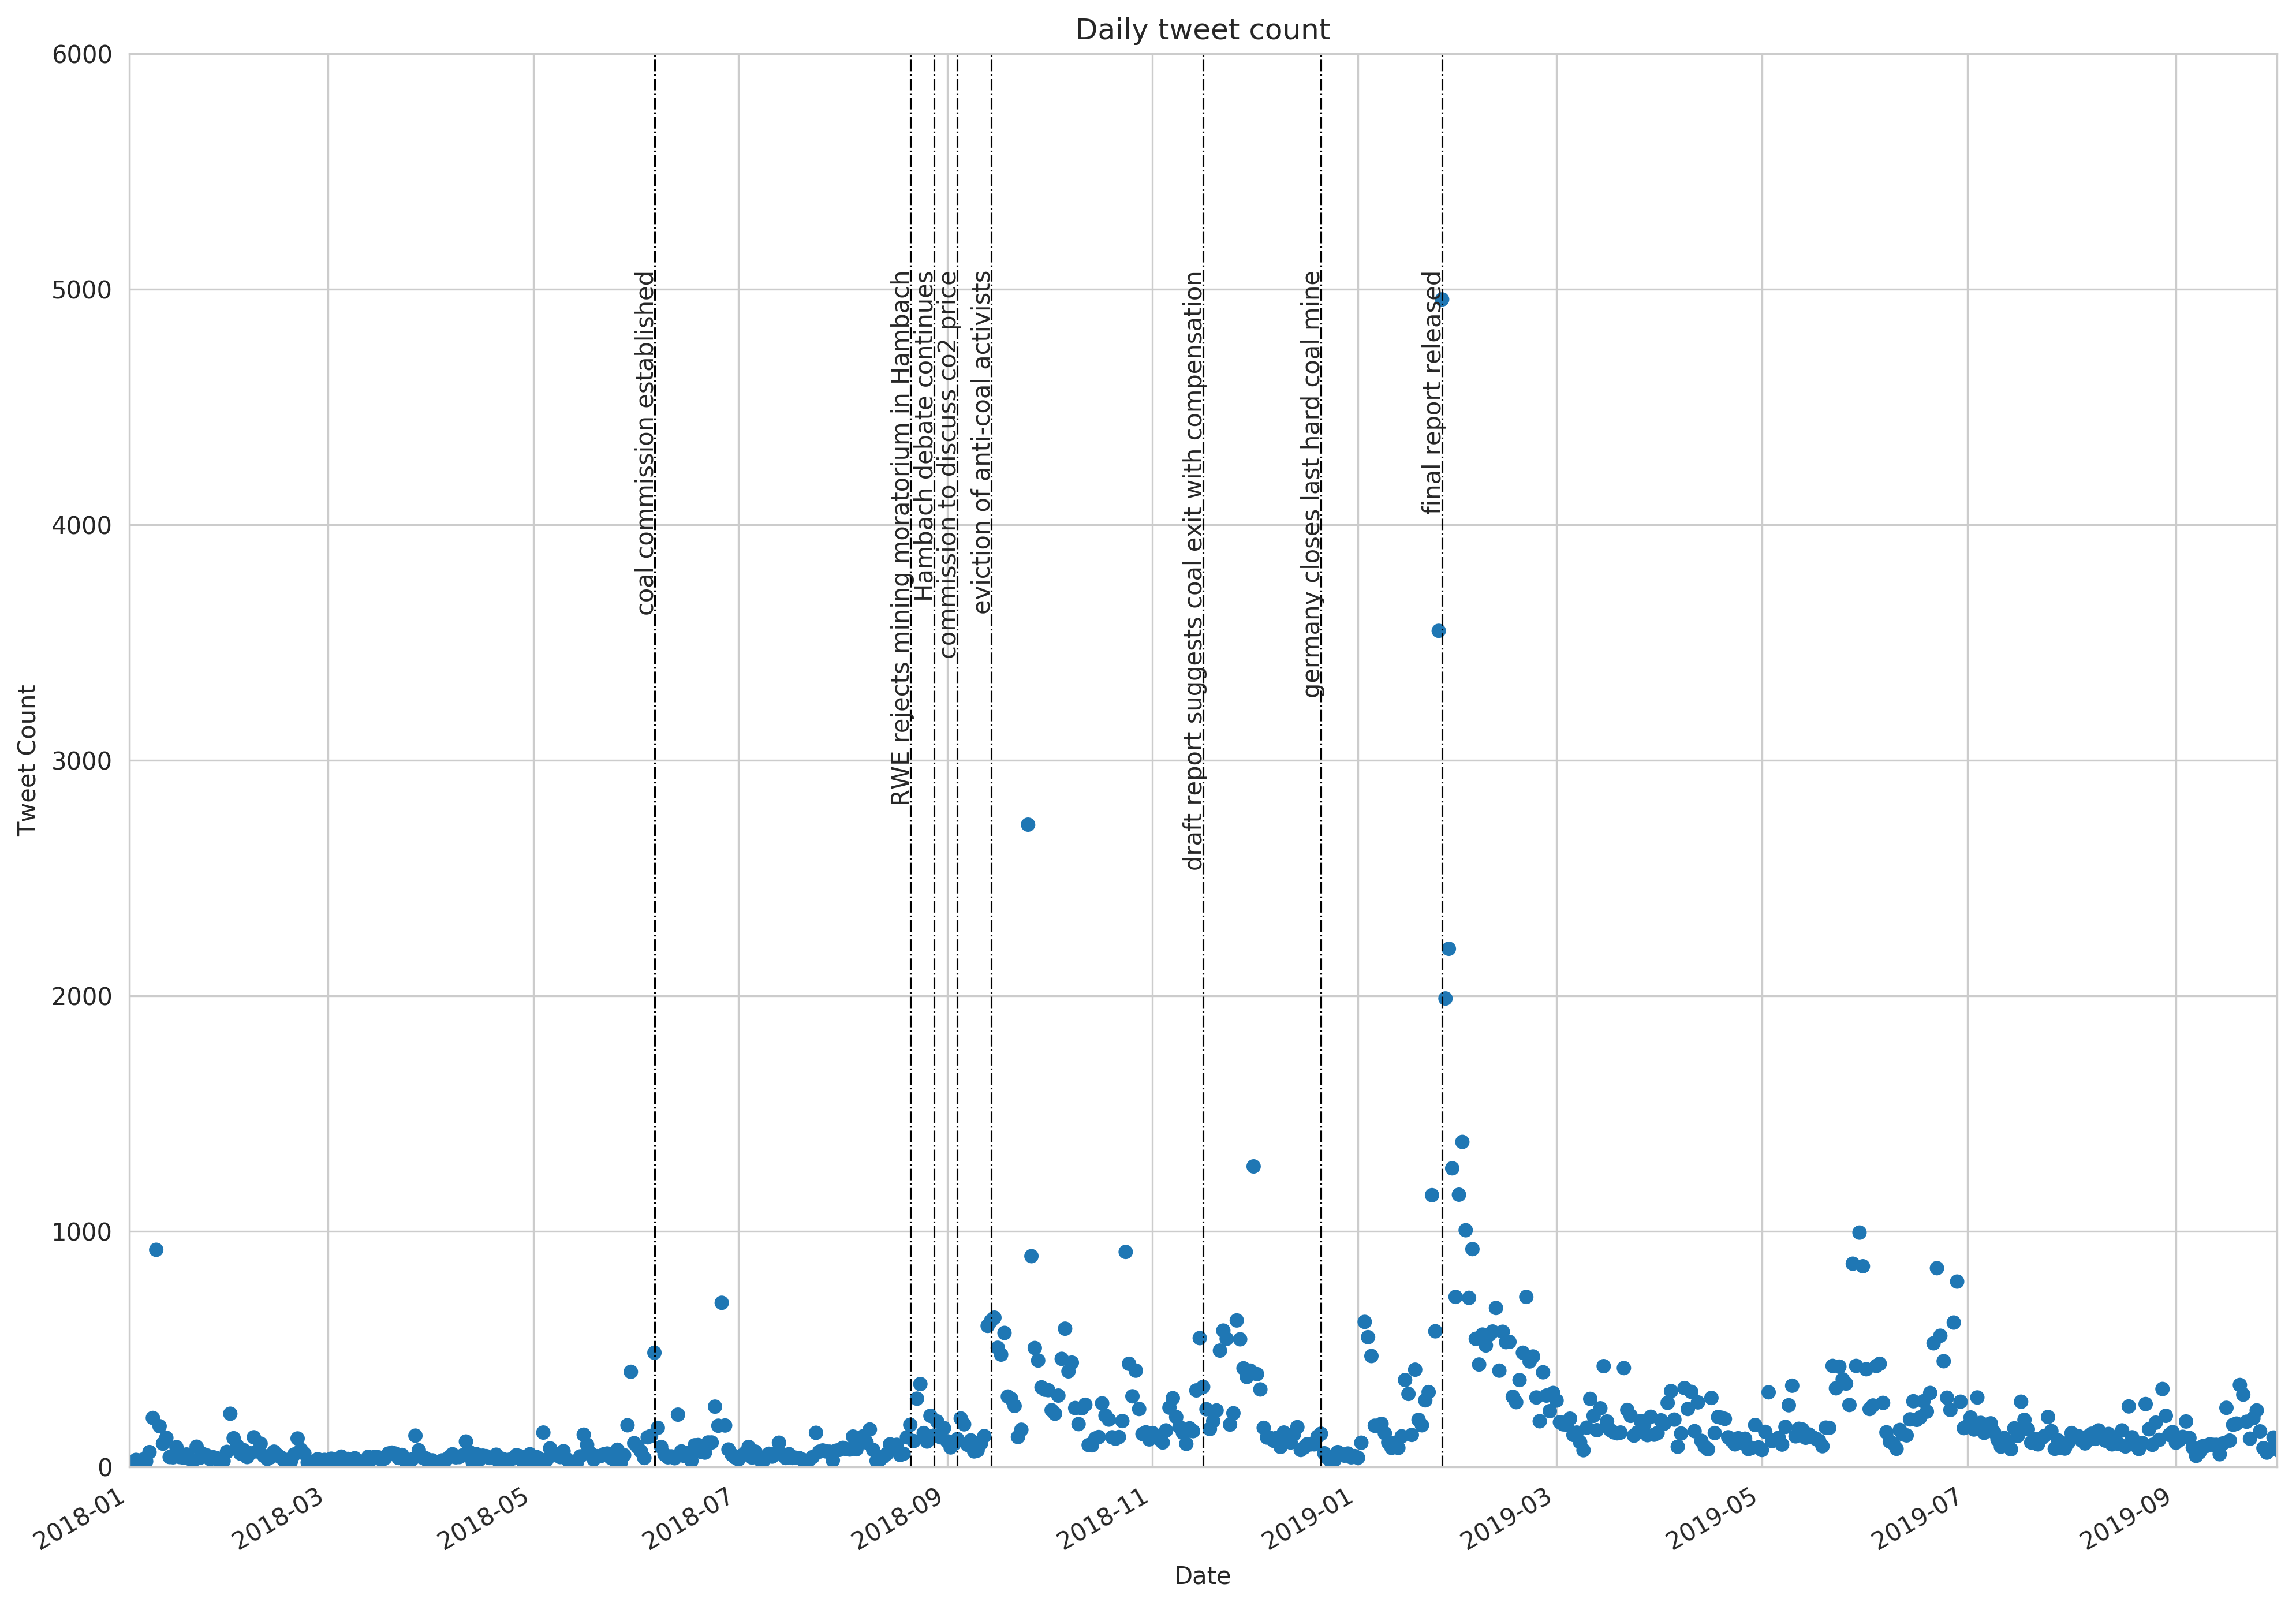
\includegraphics[width=\textwidth]{figures/sa_tweet_count_event_timeline}
	\end{center}
	\caption{Daily count of tweets throughout coal commission process against events throughout coal commission process}
	\label{fig:tweet_count_event_timeline}
\end{figure*}

\begin{figure} 
	\begin{center}
		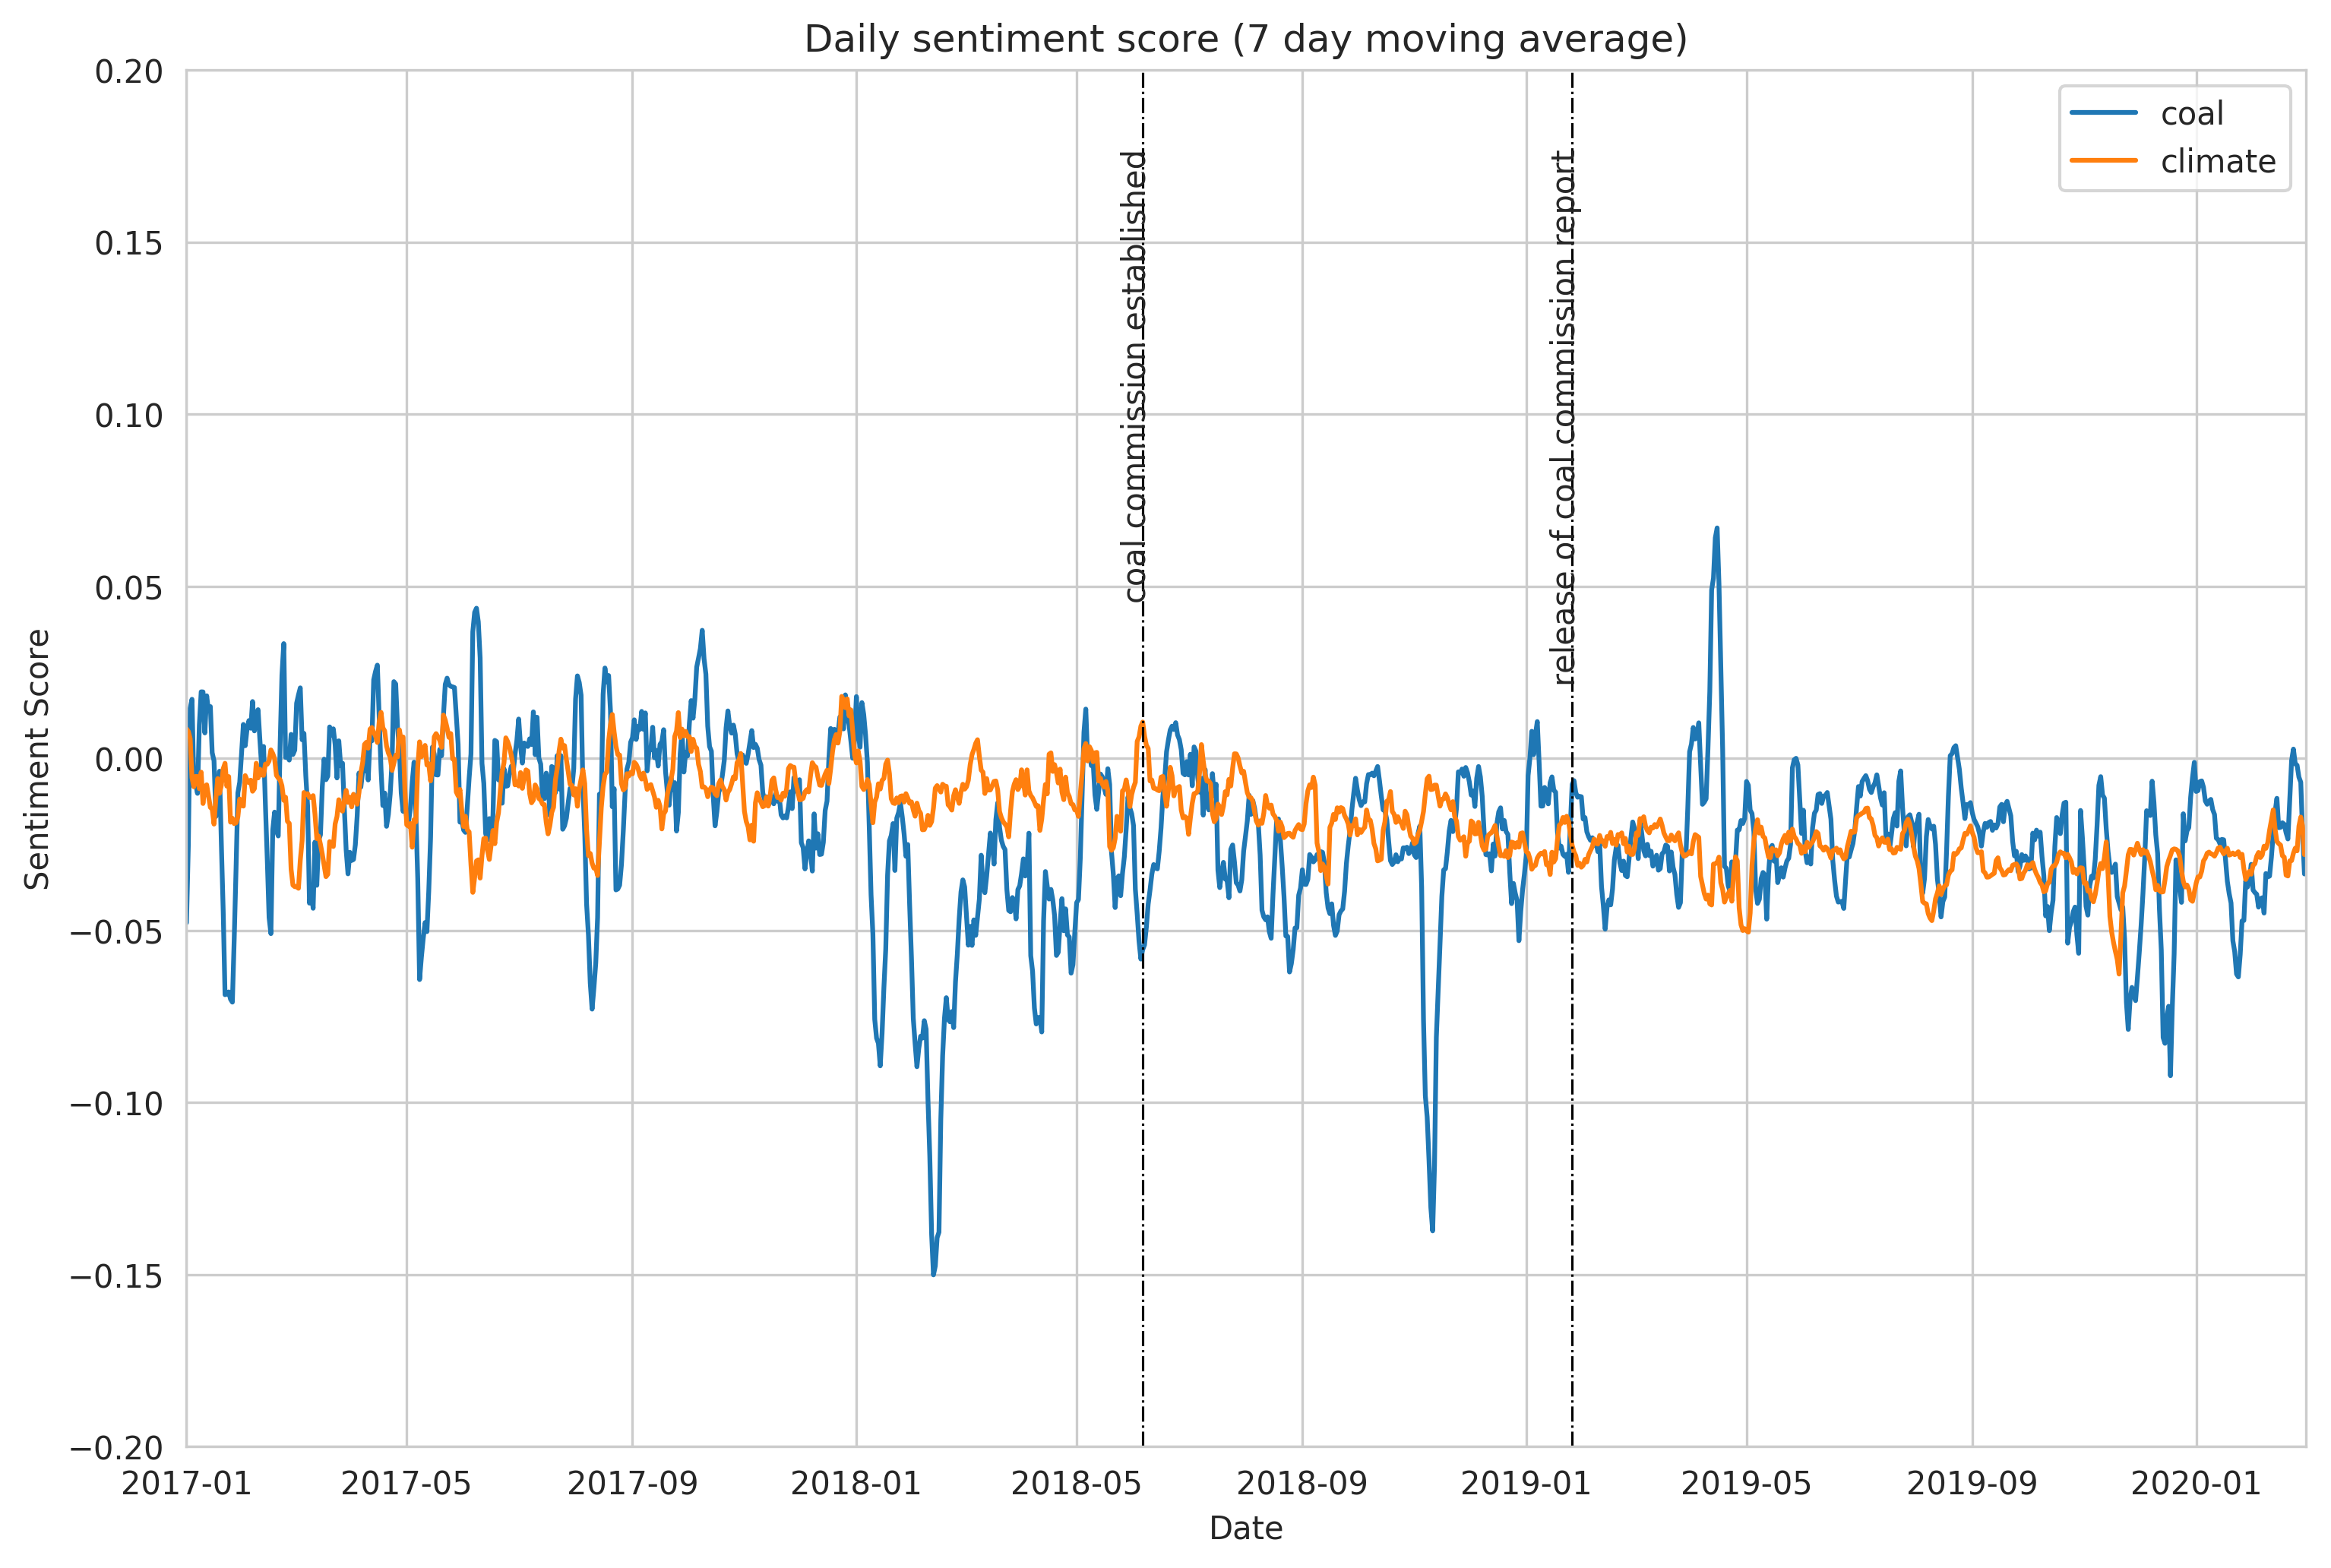
\includegraphics[width=\linewidth]{figures/sa_dailyavgsenti_7dma_baseline2}
	\end{center}
	\caption{7 day moving average sentiment score of tweets}
	\label{fig:tweet_score}
\end{figure}

Fig. \ref{fig:tweet_count_event_timeline} shows the daily count of tweets throughout the coal commission process against events throughout the same process. Fig. \ref{fig:tweet_score} shows the 7 day moving average of tweet scores in the coal and climate datasets. 

\subsubsection*{Sentiment scores against time} 
% [T: 750, C: ]
% sentiment scores against time; overall trend negative
%At a glance, the variation in sentiment scores decrease over time. This could signify the reaching of a consensus over time as opinions tend to converge, thus leading to less extreme sentiments being displayed.

Looking at Fig. \ref{fig:tweet_score}, the first observation 

% sentiment scores against time; greater variation around CC period 


\subsubsection*{Event Analysis}
% [T: 750, C: 150] 
Significant events from the coal commission process were taken from Clean Energy Wire's report on the events following the coal commission. \cite{Amelang2019} In Fig. \ref{fig:tweet_count_event_timeline} and \ref{fig:tweet_score_event_timeline}, the date of significant events are overlaid on the same plot as the daily average sentiment score of tweets. 
 
\begin{figure*}[bp] 
	\begin{center}
		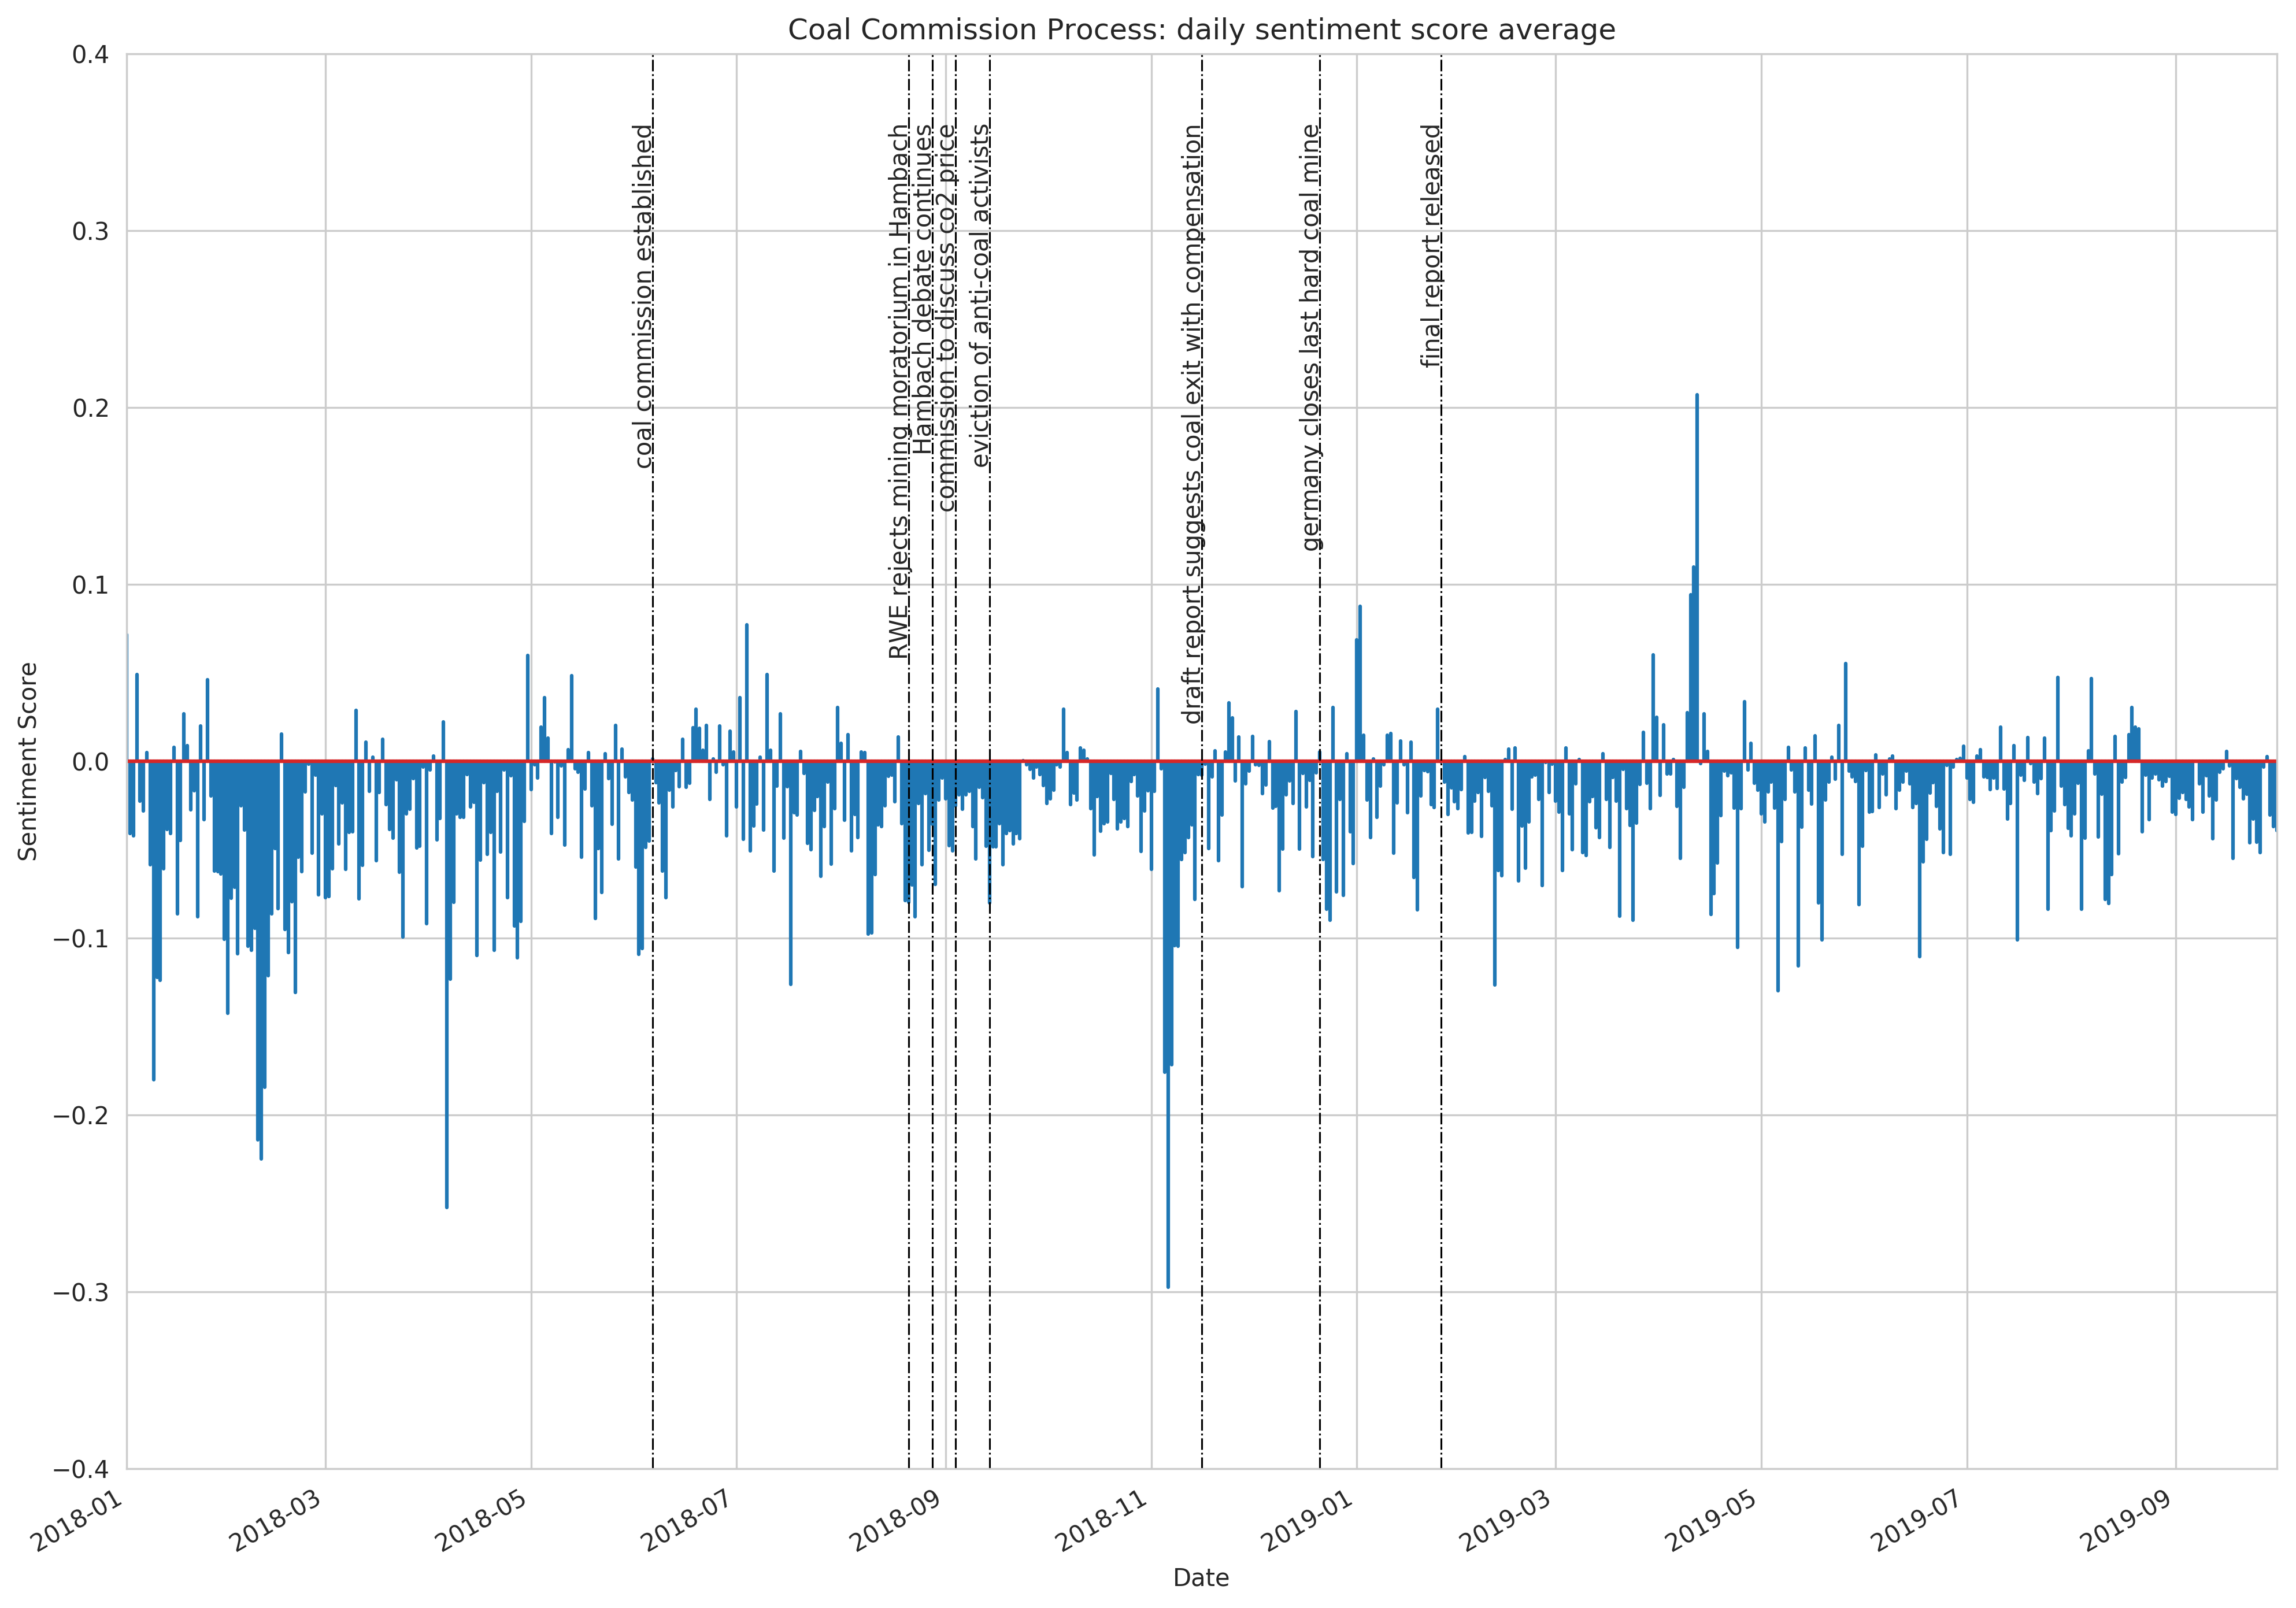
\includegraphics[width=\textwidth]{figures/sa_tweet_score_event_timeline}
	\end{center}
	\caption{Daily average sentiment score of tweets against events throughout coal commission process}
	\label{fig:tweet_score_event_timeline}
\end{figure*}

A further look at specific events in \ref{fig:tweet_count_event_timeline} show that there is an uptick in the frequency of tweets when significant events take place. In particular, the day with the most number of tweets in the dataset was on the 26th of January 2019, which was when the coal commission released its final report with recommendations on how to manage the coal phase-out in Germany. 

% positive peaks

% negative peaks 


\subsubsection*{Word Shift}
% [T: 750, C: 180]
In order to understand how the debate evolved over time, the tweet dataset used so far is split into two categories by date -- before the establishment of the coal commission and after. The tweets that were made after the coal commission was established are then analysed in comparison to the tweets that were made before the coal commission's establishment. This presents an opportunity to look at how the debate changed over time, whether the focus of the debate had changed after the coal commission began its decision-making process, and how public sentiment changed over the course of the same process. 

To look at how the language and sentiment changed over time, a method known as ``word valence shift graphs", first used in \cite{Dodds2011}, is employed. To do so, words are ranked by their absolute contributions to the change in average sentiment of one group relative to another. 



In addition, in order to understand the debate on the German coal exit on Twitter, it is necessary to compare it to other debates on Twitter. Here, the climate debate is used as a reference. 

\begin{figure*} 
	\begin{center}
		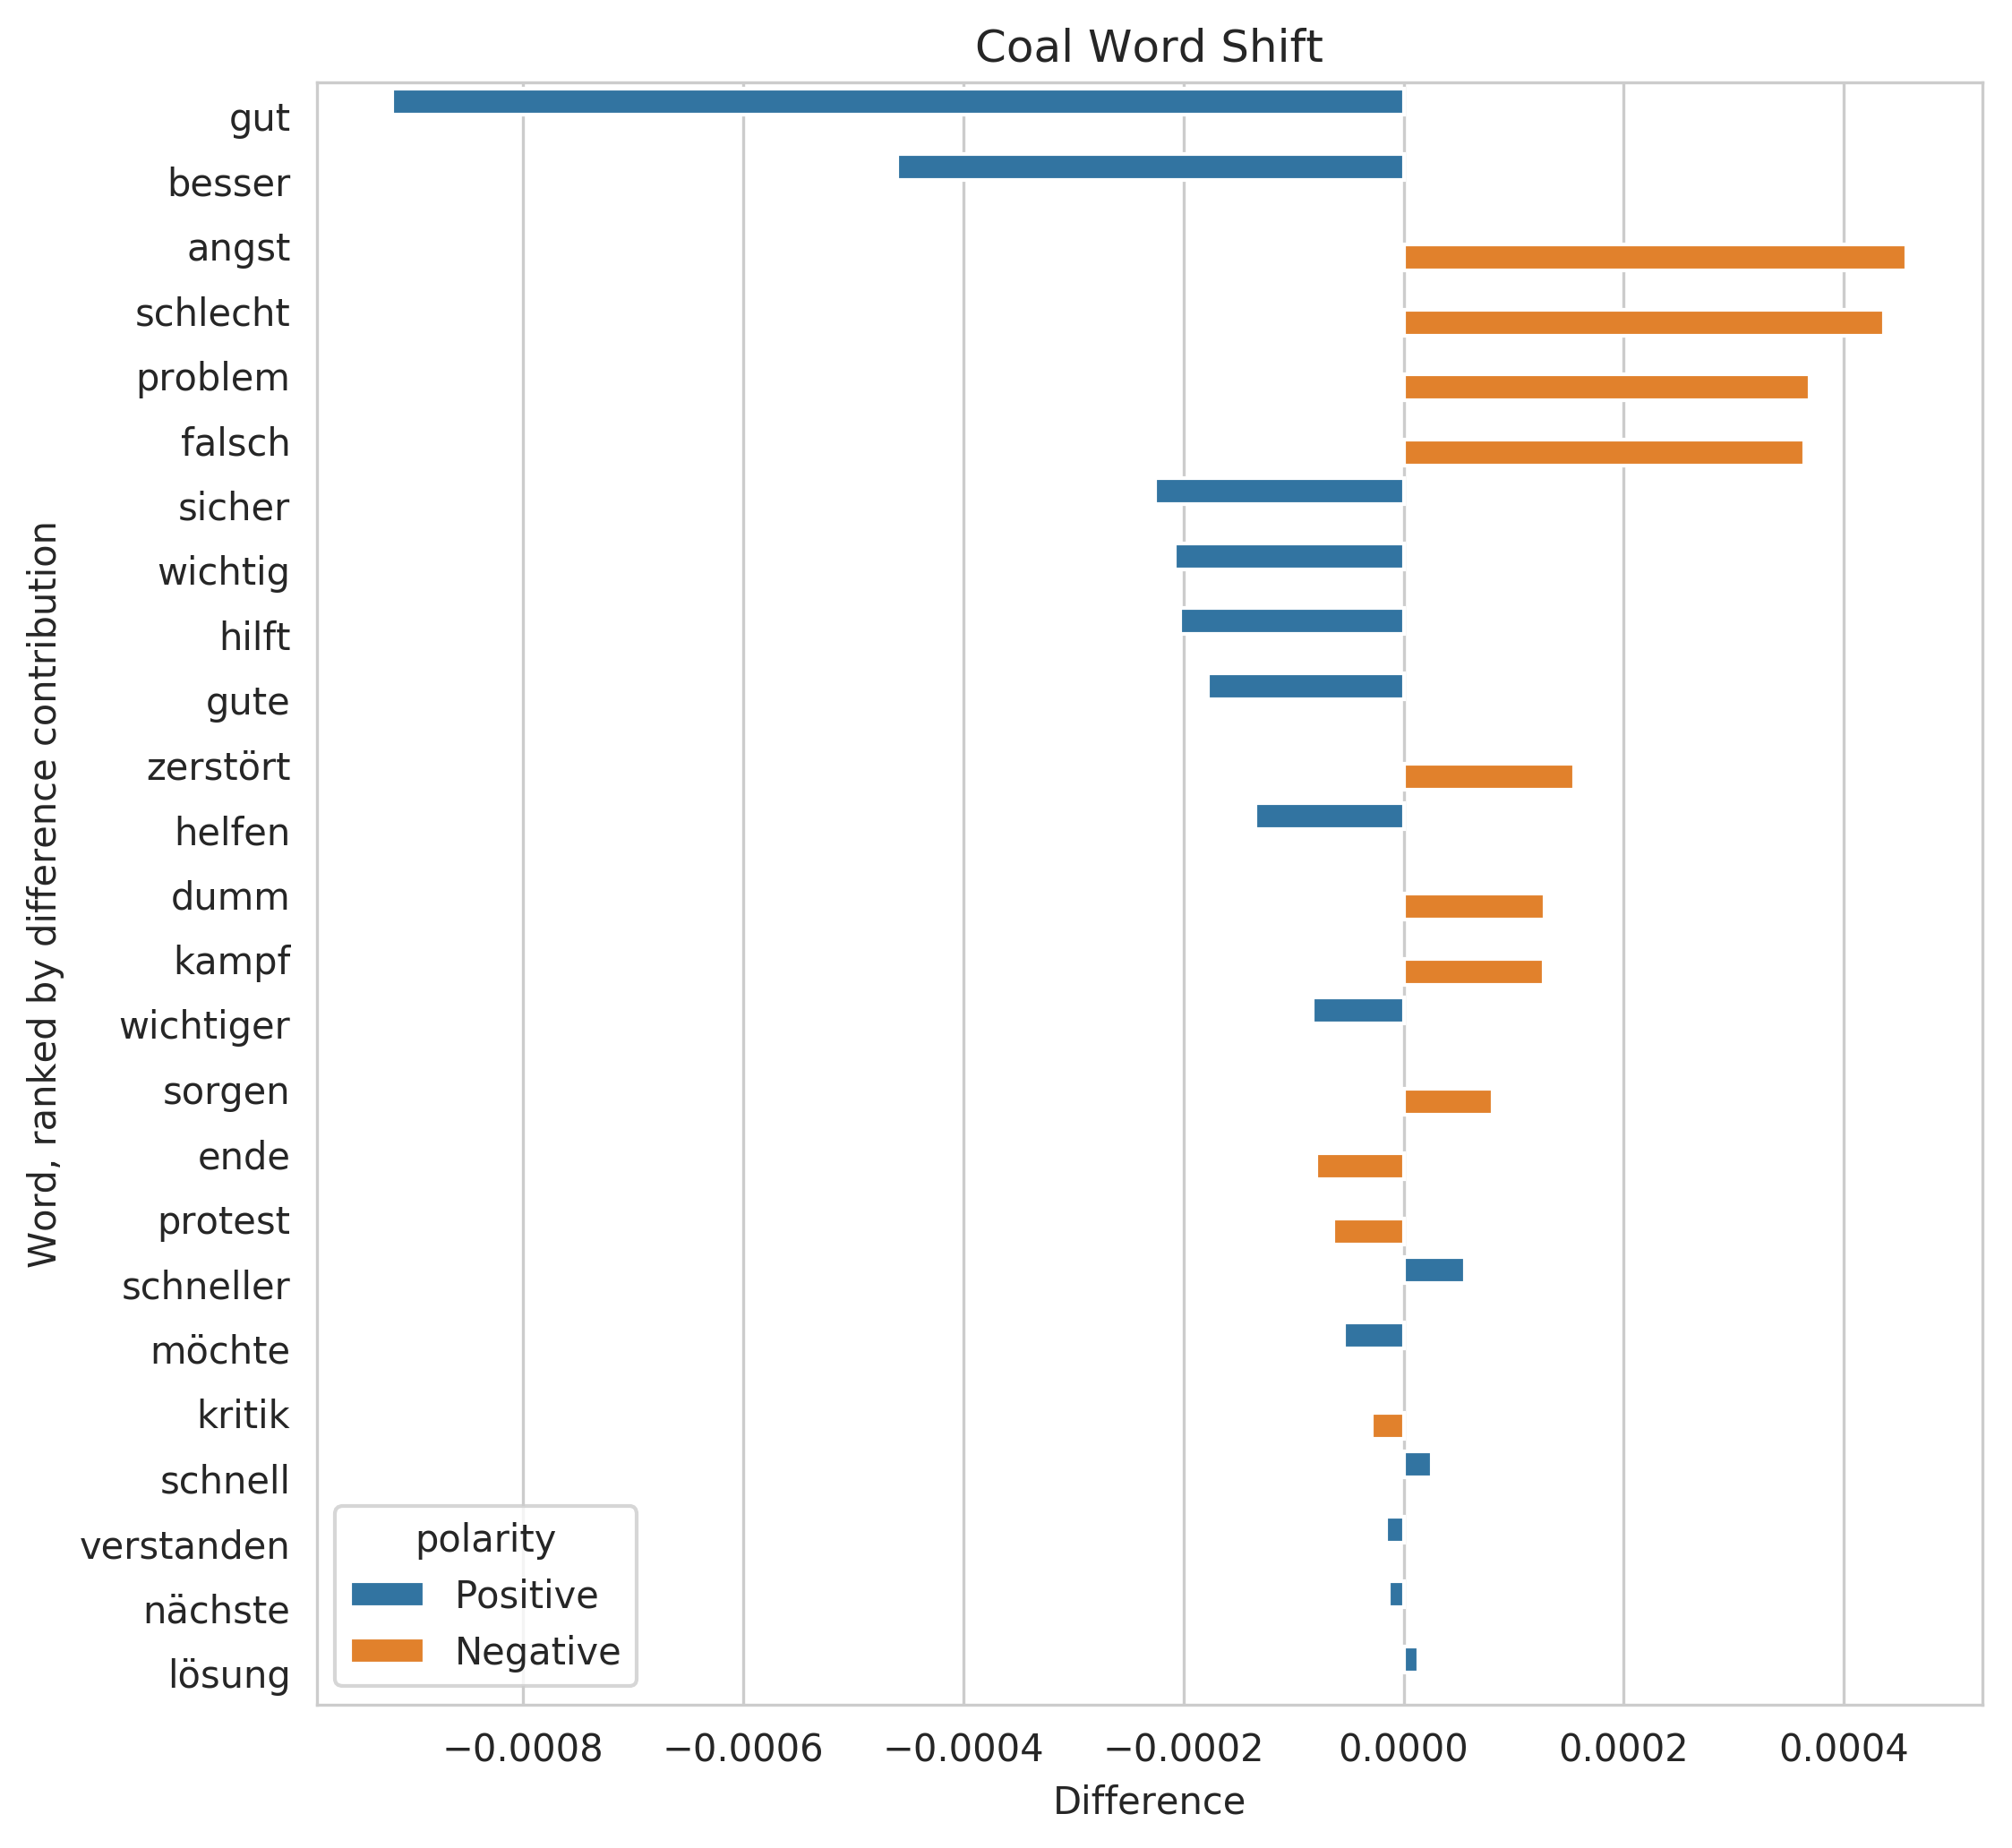
\includegraphics[width=0.8\linewidth]{figures/wordshift_coal_climate}
	\end{center}
	\caption{Word shift graph comparing coal tweets to climate tweets}
	\label{fig:wordshift_coal_climate}
\end{figure*}


\subsubsection*{Network Analysis}
% [T: 750, C: 250]
Another way of analysing the evolution of the coal debate on Twitter is to look at the retweet network of the dataset. In Twitter, a retweet refers to a re-post of a tweet, where another user chooses to share another user's tweet on their personal timeline. By taking Twitter users as nodes and retweets as edges, we can construct a retweet network and see which users retweet the most often from other users. From this, the community structure of the network can also be determined. The community structure of a network refers to the appearance of densely connected groups of vertices, with only sparser connections between groups \cite{Newman8577}. The strength of a community structure can be measured by its modularity, which is a measure of the extent to which like is connected to like in a network. It takes a value that is strictly less than 1, and it is positive if there are more edges between vertices of the same type than would be expected by chance, and negative if there are less. % cite Newman textbook here

\begin{equation}
\label{eq:modularity}
Q = \frac{1}{2m} \sum_{i,j} \left(A_{ij} - \frac{k_i k_j} {2m}\right) \delta (c_i c_j)
\end{equation} 	

\begin{figure*} 
	\begin{center}
		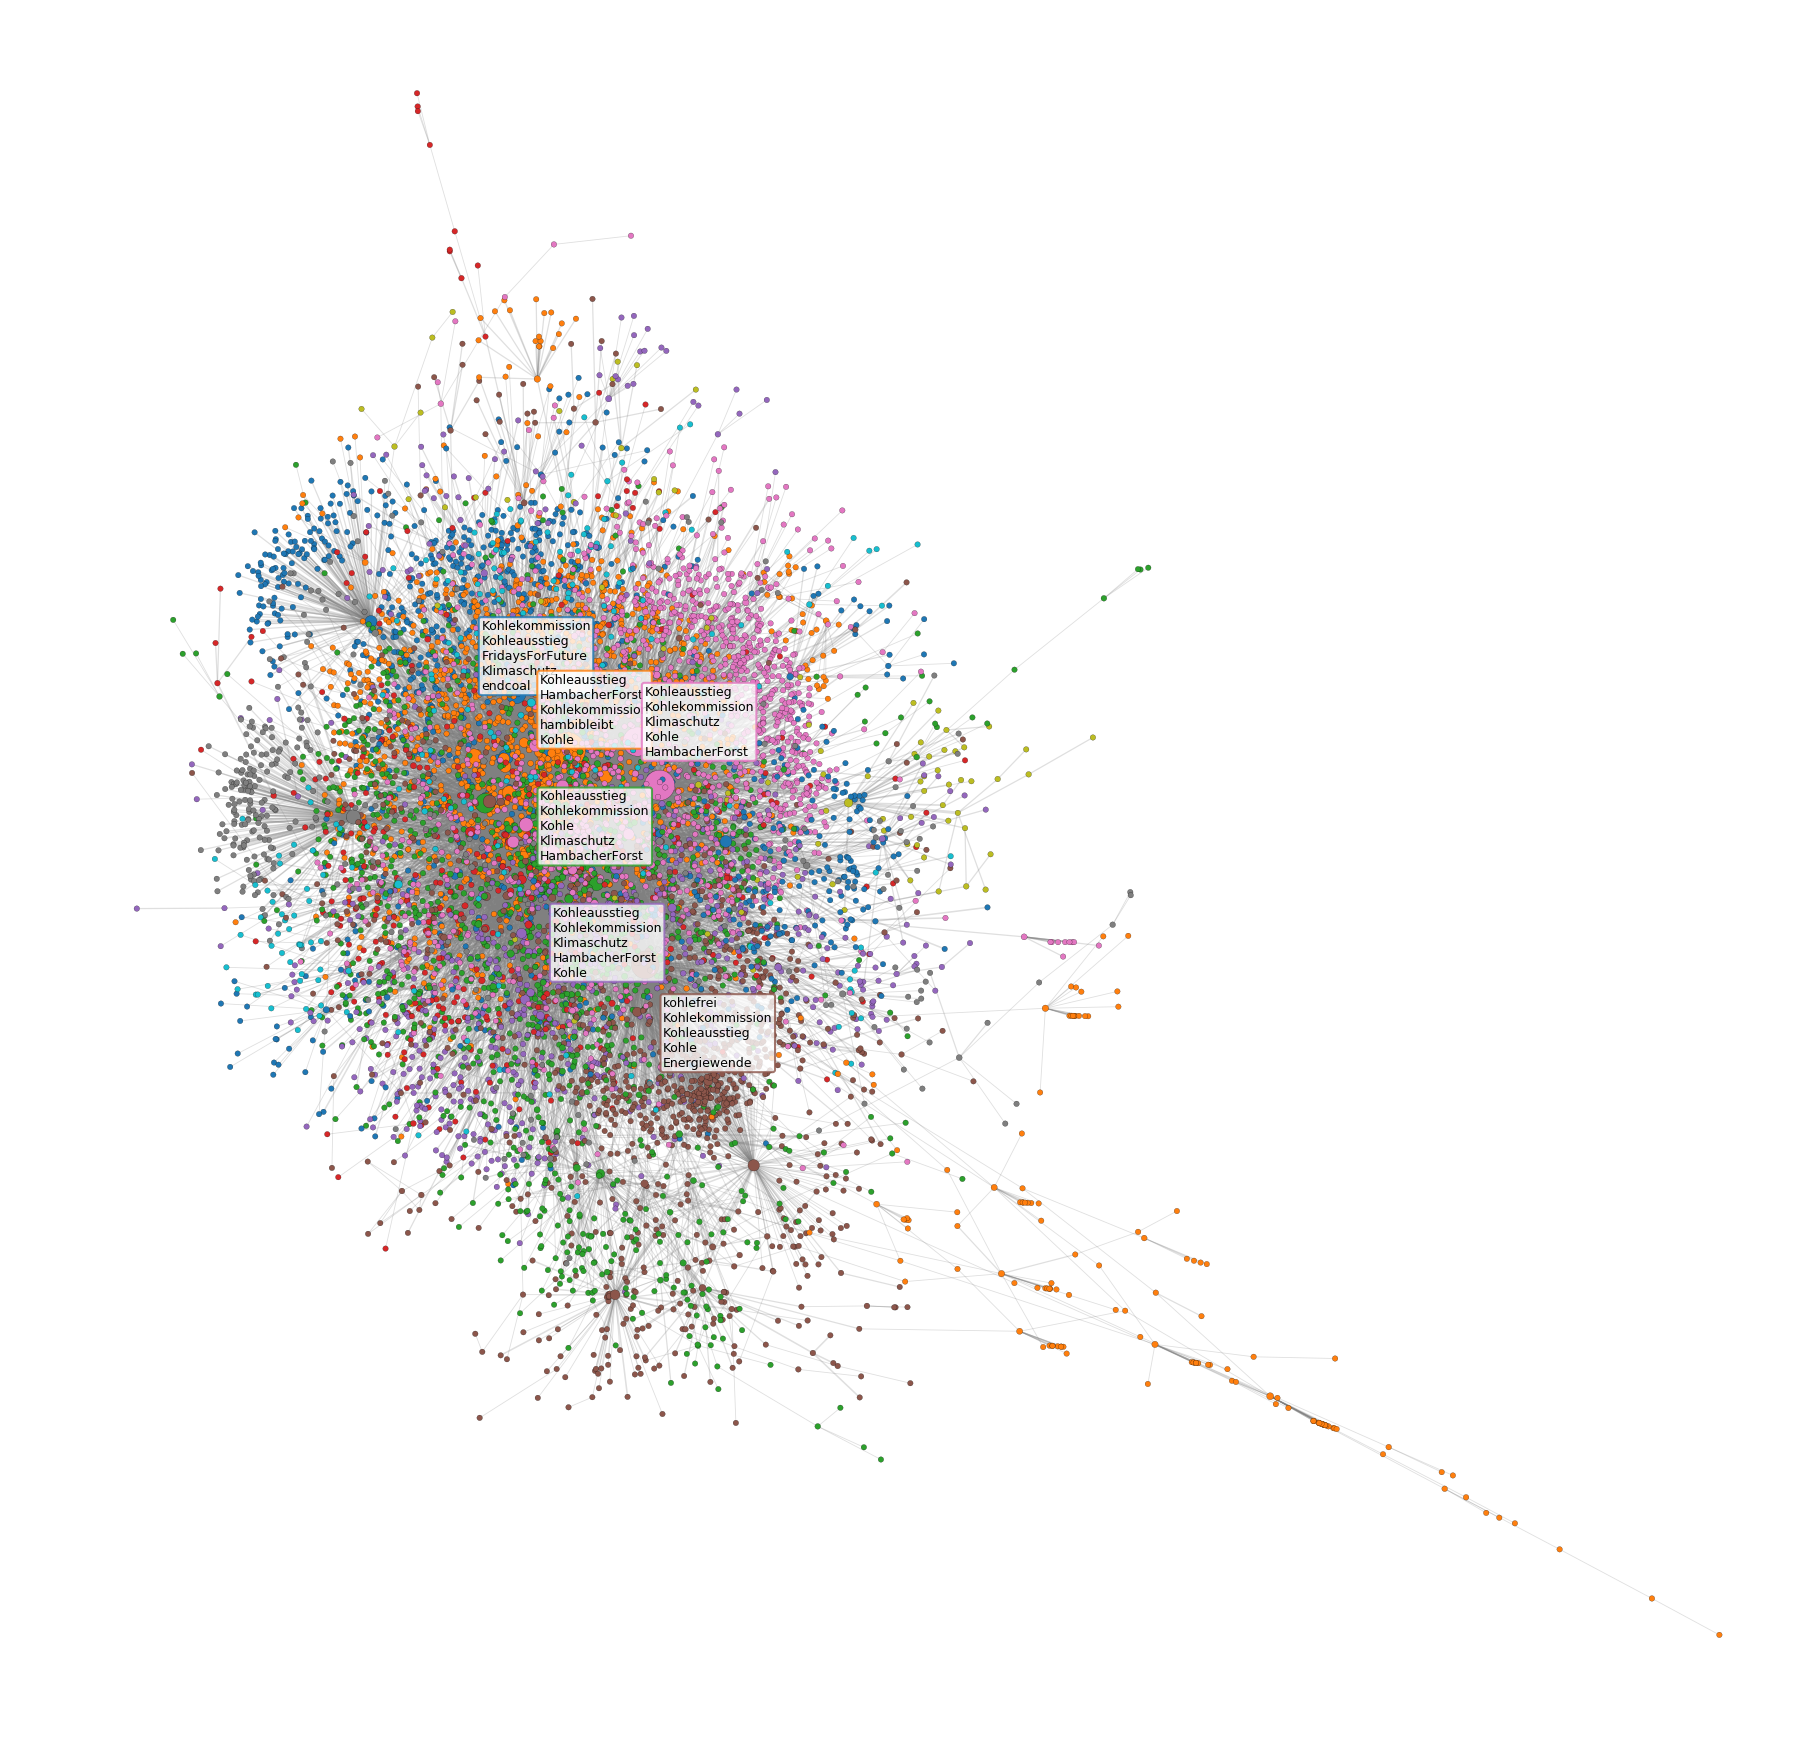
\includegraphics[width=\linewidth]{figures/rt_network_ht_period4}
	\end{center}
	\caption{Retweet network for period before release of coal commission report}
	\label{fig:rt_network_bef}
\end{figure*}	
\begin{figure*} 
	\begin{center}
		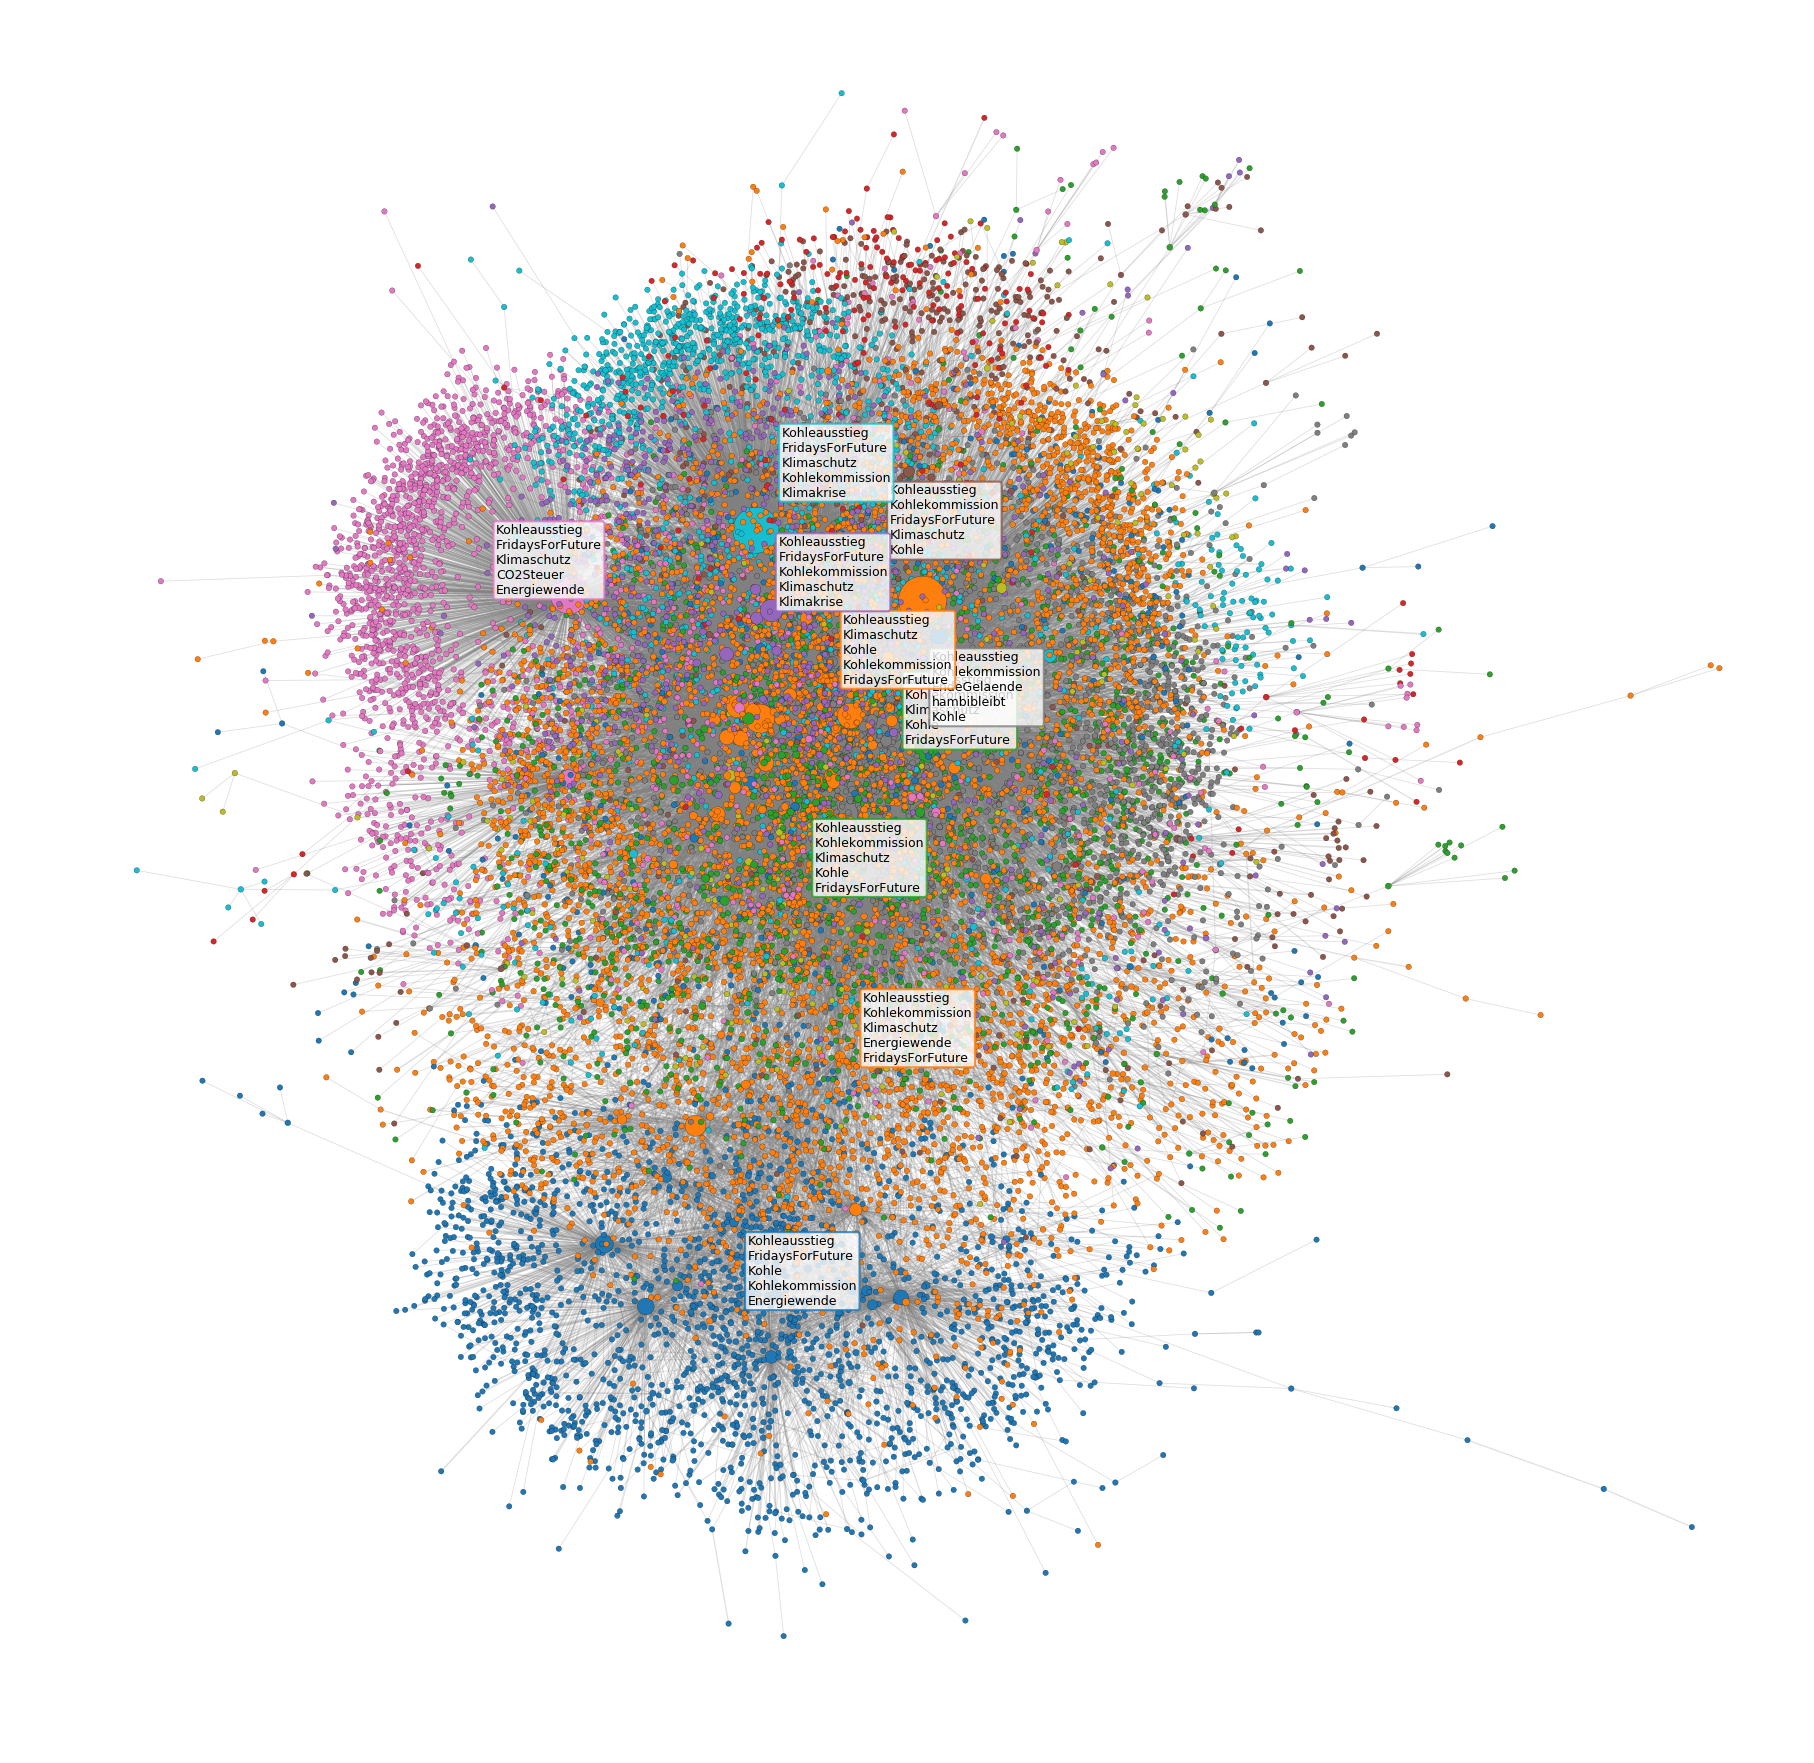
\includegraphics[width=\linewidth]{figures/rt_network_ht_period3}
	\end{center}
	\caption{Retweet network for period after release of coal commission report}
	\label{fig:rt_network_aft}
\end{figure*}

Fig. \ref{fig:rt_network_bef} and \ref{fig:rt_network_aft} show the two retweet networks of the period before and after the release of the coal commission's report respectively. 

\section*{Discussion} \label{sec:discussion}
% caveats of using dictionary methods for sentiment analysis [T: 500]

% drawbacks of using social media data, how to handle [T: 500]

% Implications of findings [T: 1K]

%%% END TEXT %%%

%\acknow{Please include your acknowledgments here, set in a single paragraph. Please do not include any acknowledgments in the Supporting Information, or anywhere else in the manuscript.}

%\showacknow{} % Display the acknowledgments section

\section*{References}
% Bibliography
\bibliography{bibliography}

\end{document}